\chapter{Discussion}

A good proxy for depositional environments must show a strong correlation to
the environments and should be insensitive to confounding influences.
Salinity would be a good proxy, because it differs substantially between freshwater, brackish and marine 
conditions, and few environments other than oceans show high salinity. However,
the salinity of their formation waters is often not preserved reliably in sediments \parencite{kharaka-2003}.
The (trace) element ratios we discuss here have been proposed in the literature as proxies
for \emph{salinity}, and thus indirectly indicate marine, brackish 
and freshwater conditions.

\section{Data quality}

Uncertainties in our measurements stem from two sources: sample preparation and analytical procedures,
and the statistical uncertainty of the measurement methods. Uncertainties due
to sample preparation and analytical procedures cannot be measured and remain unknown in most cases.
Only the \XRF instrument reports the Compton ratio as an indication whether the quality of the sample allows
reproducible measurements. 
Both, the \XRF and \ICPMS instruments report the statistical uncertainty of measurements (\cref{tab:sr-ba-table,tab:sr-ba-icpms-table,tab:s-toc-icpms-table}).

The concentrations reported by \XRF and \ICPMS differ substantially. 
\XRF reported about twice the concentrations of \acro{Ba}, and half the concentration of \acro{S}.
Because the statistical uncertainty was roughly 10\% for S and Ba for both methods, the large difference
must stem from sample preparation and analytical procedures.
While the \ICPMS method with HF digestion is known to produce reliable results,
the \XRF instrument is new, uncalibrated, was used without standards, and reported moderate to poor 
Compton ratios.
This suggests that the large discrepancy between the two methods was caused by the
uncalibrated and thus unreliable \XRF method. Therefore, the following discussion focusses
only on the \ICPMS results and skips the \XRF results.

The ROC-based best-fit algorithm combined with Youden's J statistic has limitations. 
It is an approximation that
requires that the resulting straight line always passes through at least one of the observed data points. 
When the data forms tight, well separated clusters, the derived fitting line could be far from the optimum.
This deviation from the theoretical optimum does not affect the classification of the fitted samples, 
but generalizing the result to other samples needs to be approached cautiously.

\section{Sr/Ba}

Strontium and Barium are both alkaline-earth elements.
The radius of the Sr atom is slightly larger than that of \acro{Ca}, 1.26\,\AA\ vs. 1\,\AA, and slightly smaller 
than potassium (\acro{K}, 1.38\,\AA). Sr can
substitute for \acro{Ca} and the monovalent \acro{K} in some minerals. The radius 
of \acro{Ba} (1.42\,\AA) is too large to substitute
for \acro{Ca} in most crystal lattices, particularly in calcite~\parencite{housecroft-chemistry}.
Under chemical weathering Sr preferentially leaves the crystal lattice. It is
mobile, leading to higher Sr concentrations in the oceans compared to freshwater~\parencite{brand-veizer-1980}.
The main sink for Sr in the oceans is substitution for Ca in biogenic carbonates, and in brines with high Sr concentrations,
the formation of strontianite (SrCO$_3$)~\parencite{banner-hanson-1990,wei-2020}.

Ba in silicate minerals weathers less readily than Sr, the main Ba weathering flux comes from barite (BaSO$_4$)
and witherite (BaCO$_3$)~\parencite{wei-2020}.
Due to the very low solubility of its sulphates and sulphides, Ba is not mobile and occurs only in very low 
concentrations in all waters. In freshwater, Ba is transported primarily 
adsorbed to clay minerals. With increasing salinity, ion exchange desorbs Ba from the clays~\parencite{wei-2020}.
Most Ba in the oceans precipitates as
barite (BaSO$_4$) due to the high concentration of SO$_{4}^{2-}$ in the oceans.

The data in \cref{fig:sr_ba_crossplot} are not clearly
separated into marine and freshwater sectors, and the thresholds for the \acro{Sr}/\acro{Ba}
ratios proposed by \textcite{wei-2020} fit our samples poorly~(cf. \cref{tab:icpms-classification}).
The misfit between our data and the model from \textcite{wei-2020} is caused by our \acro{Sr} values being
considerably
higher than the mean values from \textcite{wei-2020} (\cref{fig:sr-ba-wei}). There are several possible
explanations for this. 

\begin{table}[b!]
    \centering
    \caption{Classification of our samples into marine (M), brackish (B) and freshwater (F) according to different methods.
    Where applicable we compare our data against the classification criteria of \textcite{wei-2020}. 
    Geological map classification based on \textcite{Linth_Map}.}\label{tab:icpms-classification}
    \input{temp/icpms-classification-table.txt}
\end{table}

% First, \cref{fig:sr-ba-wei} shows that there are some outliers of marine sediments with high \acro{Sr}
% values in the dataset from \textcite{wei-2020}, and the case study discussed in detail by them
% concludes that the samples have abnormally high Sr values without an explanation. 
% Therefore, it is possible that our samples simply have
% abnormally high \acro{Sr} values that the global model cannot explain. 

First, it is possible that the rocks that we classified as freshwater sediments are
actually sediments from brackish or marine environments.
However, the S/TOC data discussed in the next section contradicts this interpretation.

Second, \textcite{wei-2020} state that
carbonate-rich rocks may have high concentrations of \acro{Sr}, because \acro{Sr} can substitute
for \acro{Ca} in calcite (up to 10\,000\,ppm) and aragonite (up to 80\,000\,ppm).
However, such high concentrations are only observed in biogenic carbonates and calcite recrystallized from aragonite, 
but not carbonates precipitated from solution (Picotti, V., 05/2026, personal communications). Mud-
and siltstones contain carbonates only as cement, which is precipitated, not biogenic. 

\textcite{banner-hanson-1990}
developed a theoretical model to estimate the equilibrium concentrations of Sr between precipitated calcite and water.
As an example, in solutions with 10\,ppm Sr, the equilibrium concentration in calcite is 200\,ppm. 
Given typical concentrations of Sr in natural waters (mean 40\,ppb in freshwater and 8\,ppm in seawater)
\parencite{musgrove-2021,wei-2020}, the model predicts Sr concentrations below 200\,ppm in carbonates.
Our measured concentrations are much higher than 200\,ppm.
Considering that the carbonate content in our
samples is only 13--44\%, carbonates with an expected Sr concentration less than 200\,ppm cannot 
be the only explanation for the high Sr concentrations.

\begin{figure}
    \centering
    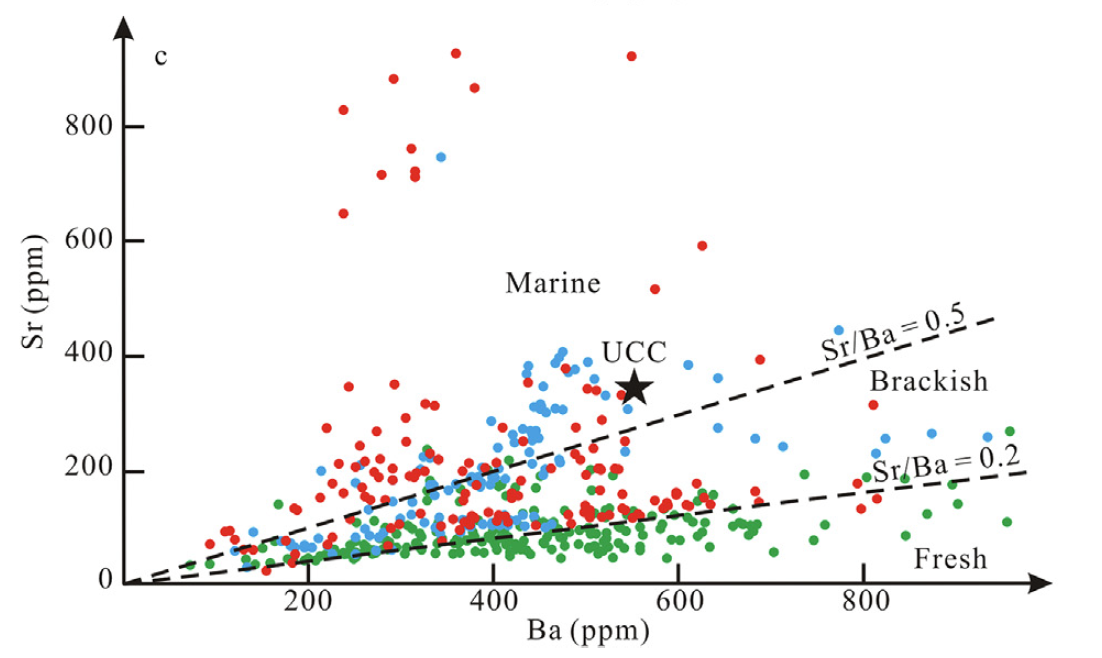
\includegraphics[width=0.5\textwidth]{img/sr-ba-wei.png}
    \caption{Sr/Ba cross-plot of all data from \textcite{wei-2020}. The mean Sr value is approximately 200\,ppm.
    Colour coding: freshwater green, brackish blue, marine red.}
    \label{fig:sr-ba-wei}
\end{figure}

\begin{figure}
    \centering
    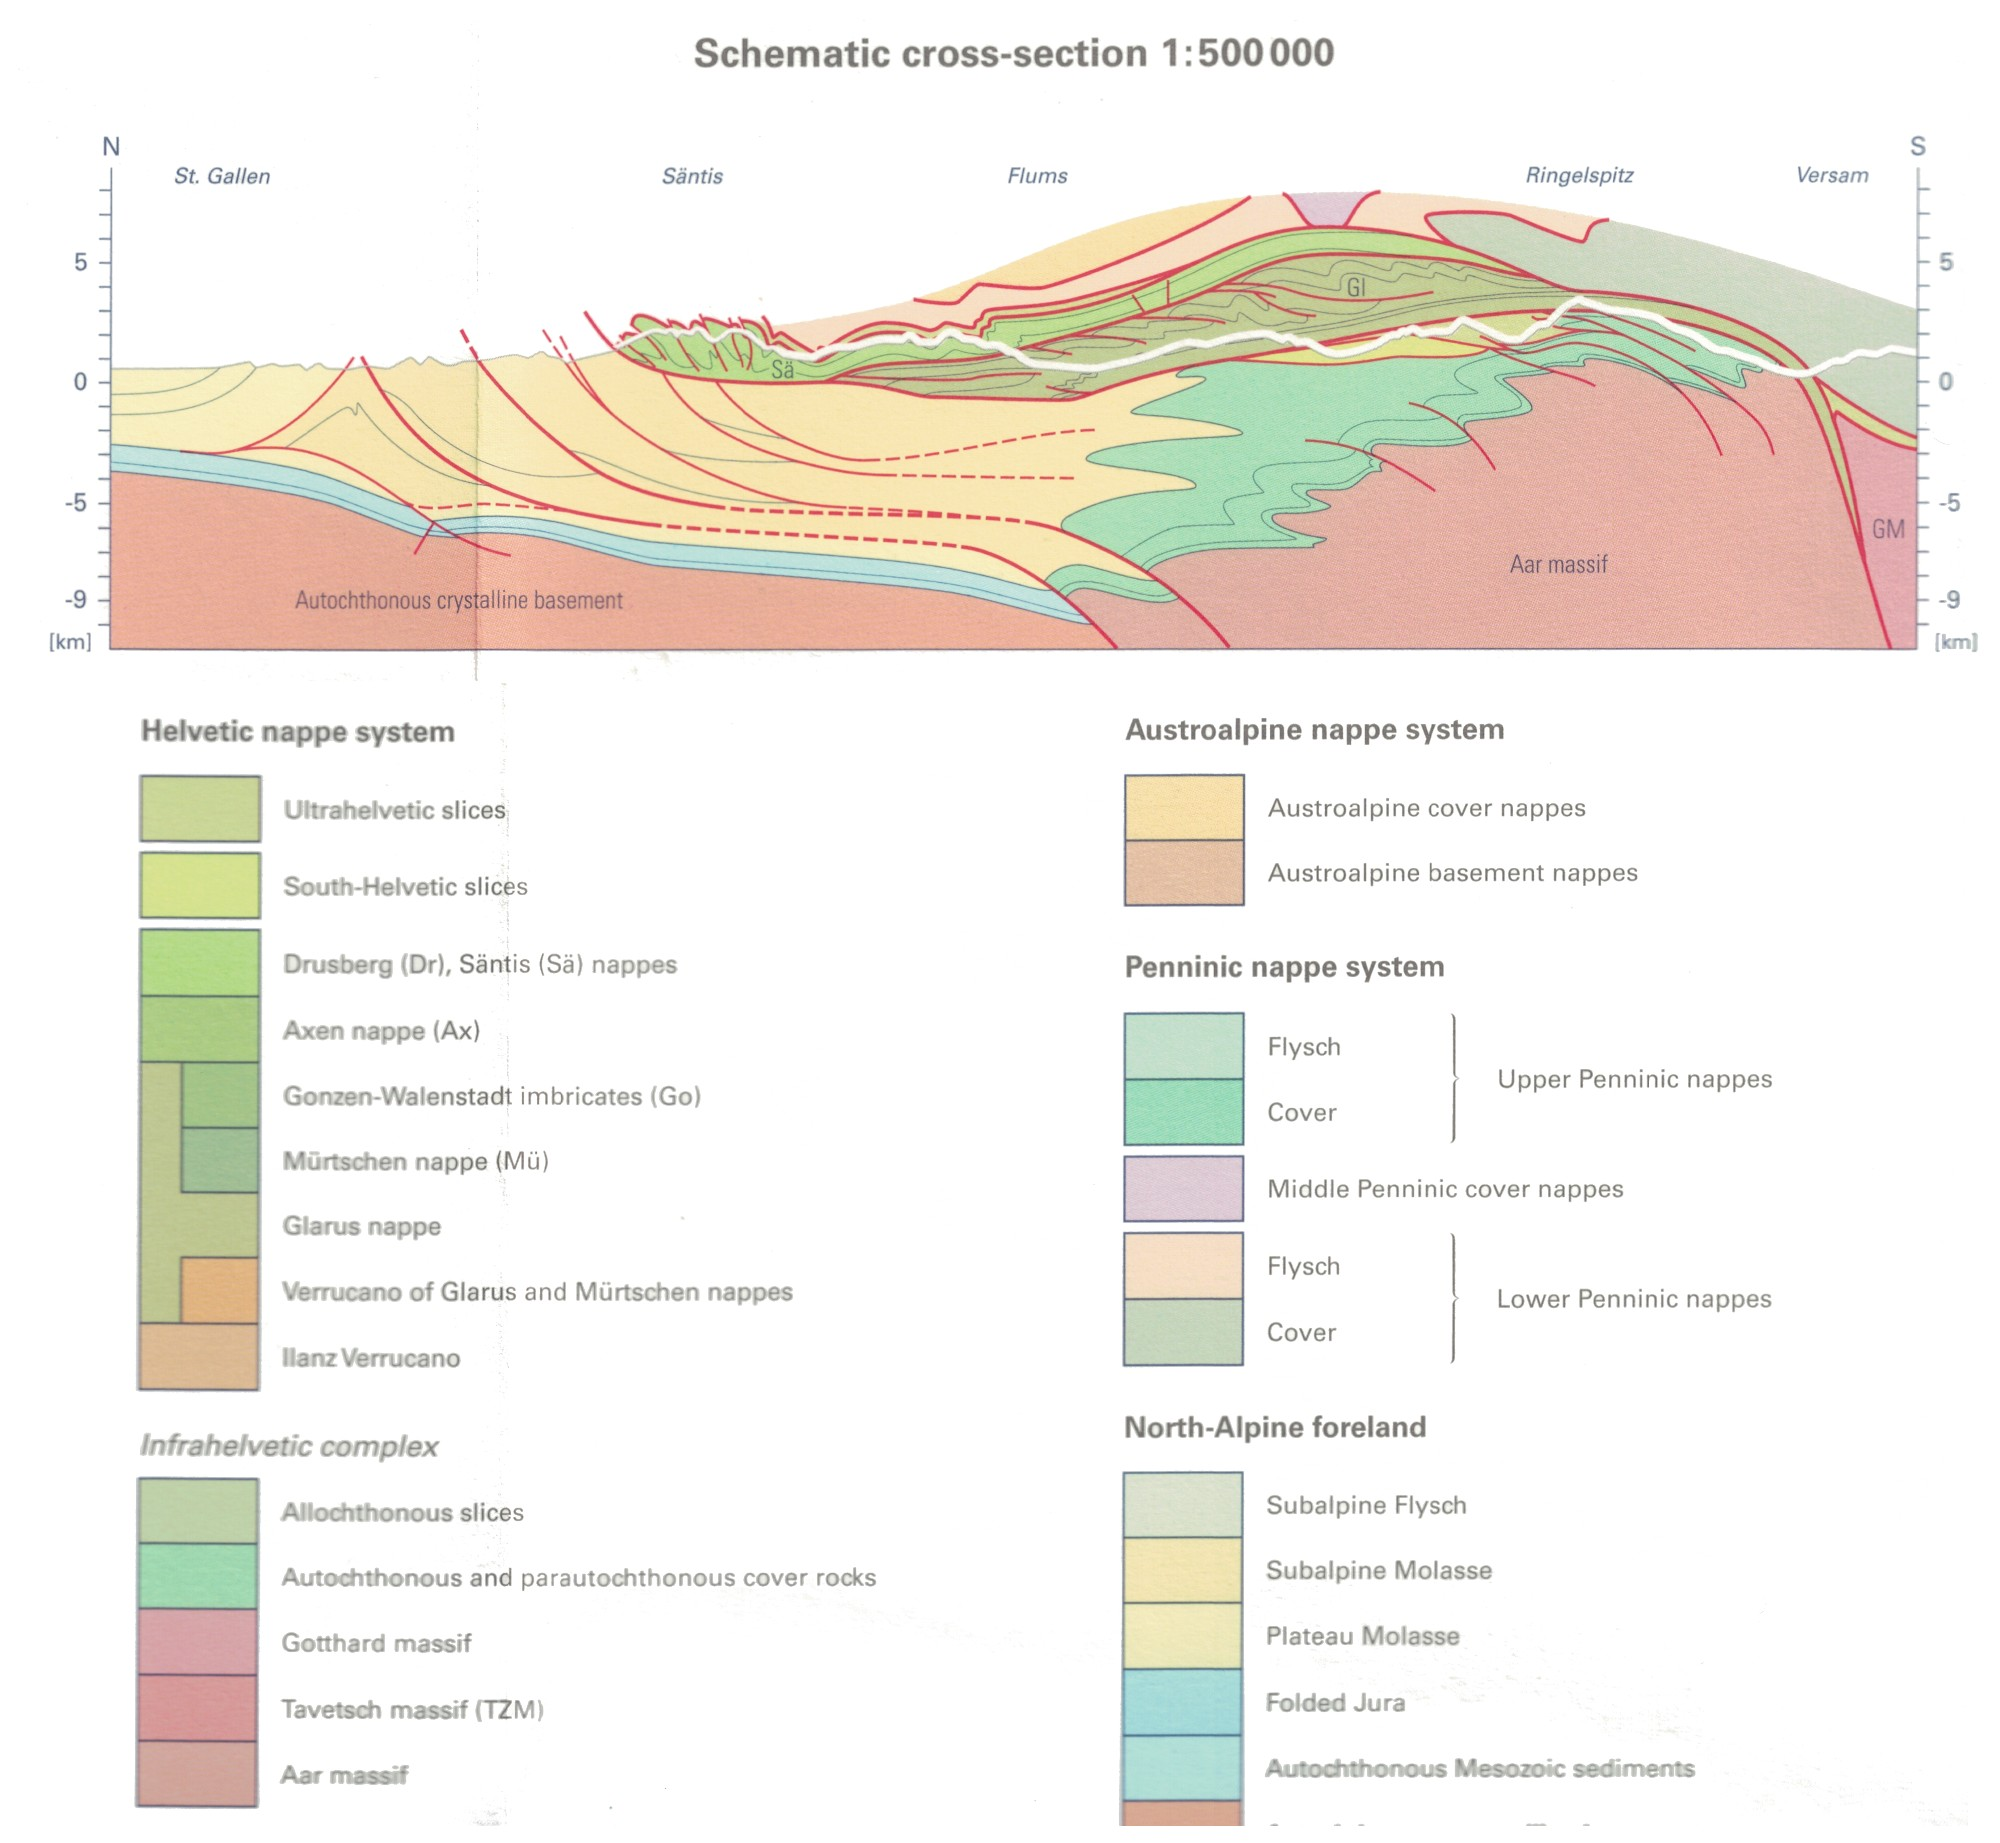
\includegraphics[width=.95\textwidth]{img/profile_large.jpg}
    \caption{Schematic cross-section through the SMB and subalpine molasse in the study area. The 
    subalpine molasse originally rests on the Mesozoic sediments, and potentially early Cenozoic
    sediments. The study area lies at the surface contact between the Subalpine Molasse and overthrust
    Helvetic nappe. Source: \textcite[map sheet 33]{helvetic-map}}
    \label{fig:overview-profile}
\end{figure}

Third, \textcite{kharaka-2003} studied deep water
bodies, which typically have very high amounts of \TDS. They found that
\acro{Sr} concentrations correlate strongly with \TDS and can reach several hundred ppm in
those deep brines. These high \TDS values usually occur in aquifers that are in contact with
limestone and/or evaporites like gypsum and anhydride.

The \UMM was deposited on top of the Mesozoic sediments that underlie the entire \SMB 
(\cref{fig:overview-profile}, \textcite{helvetic-map}). Locally, the \UMM may lie on the
marls of the late Eocene Stad and Euthal formations \parencite{Ibergeregg_Text}, but in Eastern
Switzerland, the molasse usually rests on the Jurassic Malm limestones \parencite{chevalier-molasse-2010}.
The Stad and Euthal formations are rich in fossils \parencite{Einsiedeln_Text}, 
and the upper Malm limestones represent a carbonate platform \parencite{chevalier-molasse-2010}, 
so they may contain very high concentrations of 
\acro{Sr}. When these sediments were buried under the UMM, compaction may have expelled the briny pore waters,
which then would have risen upwards and transported the contained Sr into the UMM sediments, where they
provided the high
Sr concentrations in the pore waters from which the calcite cement precipitated~\parencite{kharaka-2003}.

% \begin{table}
%     \centering
%     \caption{Classification of our rocks samples into marine (M), brackish (B) and freshwater (F) according to different methods.
%     Where applicable we compare our data against the classification criteria of \textcite{wei-2020}. 
%     Geological map classification based on \textcite{Linth_Map}.}\label{tab:xrf-classification}
%     \input{temp/xrf-classification-table.txt}
% \end{table}

Overall, our data suggest that without calibration to local conditions, e.g. by using a few standard samples
of known origin to define the classification threshold, the Sr/Ba ratio cannot be used reliably for the classification
into marine/freshwater conditions. 

\section{S/TOC}

Sulphur occurs in many minerals and is a major constituent of organic matter.
In aqueous solution S usually exists in the oxidized form of sulphate (SO$_4^{2-}$), which is
highly mobile and is transported to the oceans. The average sulphate concentrations are
27\,ppm in freshwater and 2900\,ppm in seawater \parencite{wei-2020}.
This difference in concentration is reflected in the amount of S preserved in sediments.

The preservation of \acro{S} and organic carbon in sediments is mainly controlled by 
bacterial sulphate reduction in anoxic sediments rich in organic matter~\parencite{berner-raiswell-1983}.
During this process, sulphate is reduced to sulphide and organic matter is destroyed. 
The sulphide and the surviving organic matter are deposited as metal sulphides and \TOC, respectively.
\textcite{berner-raiswell-1983} estimate the S/TOC ratio in marine sediments to be around 0.33 and
in freshwater 0.1 or even less. These trends are shown as dark grey lines in \cref{fig:toc_s_crossplot}.

Our data forms well separated clusters and fits the model by \textcite{wei-2020} 
reasonably well~(\cref{fig:toc_s_crossplot}), again except for sample JWL 1.
The best fit line lies in the middle of the brackish sector from \textcite{wei-2020}, 
and between the general trends proposed by \textcite{berner-raiswell-1983}. 
Overall, the S/TOC ratio separates marine and freshwater sediments
clearly and appears to be suitable for classification, even
without local calibration.

\section{A marine transgression?}

Sample JWL 1, a USM sample according to \textcite{Linth_Map}, was classified as marine
by all methods and thresholds from the literature as well as our best fit 
thresholds~(\cref{tab:icpms-classification}). 
It exhibits a much higher S/TOC ratio than all other samples. 
While it is possible for such an S/TOC ratio to occur in lake sediments with euxinic conditions 
in the water column, such lakes are rare \parencite{berner-raiswell-1983}. It is 
far more likely that the high S/TOC is a strong marine signal.

All marine samples contain
significantly more carbonate than freshwater samples. The exception are our two reference
samples for flysch (JWL 6) and \OSM (JWL 7), where the order is reversed (\cref{fig:carbonate}).
This is consistent with their depositional settings:
flysch is a detrital deep marine sediment, less likely to contain carbonate, and the \OSM is known to contain 
a lot of freshwater carbonate (e.g. \parencite{gubler_2009e}). The climate also differed 
between the Eocene flysch and the late Miocene \OSM deposition,
which likely influenced the overall chemistry of the sediments \parencite{schlunegger_possible_2007}.
JWL~1 has the second-highest carbonate content of all samples, which supports its interpretation as a 
marine sediment.

JWL~1--3 were collected from the same \USM outcrop (\cref{fig:log_L1}).
Our measurements confirm that JWL~2 and 3 are freshwater sediments, and suggest that JWL~1 is a marine sediment.
Whether this represents a period of marine transgression or whether this layer was folded in between the
freshwater sediments during the period of strong tectonic deformation of the subalpine molasse
is a question we cannot answer with the geochemical data obtained in this study.

The mudrocks above the gap in the outcrop (\cref{fig:log_L1}), 
especially the bed in directly below the overlying sandstone,
show fractures and slickensides indicating fault movement. 
This raises questions about the nature of the unexposed interval. 
It is more weathered and overgrown: is that because the rock is more fractured, 
like a fault gouge, or is it made of softer, more easily weathered sediments than the surrounding
outcrop? Indications of where exactly the change in depositional environment happened may be buried there.

\begin{figure}
    \centering
    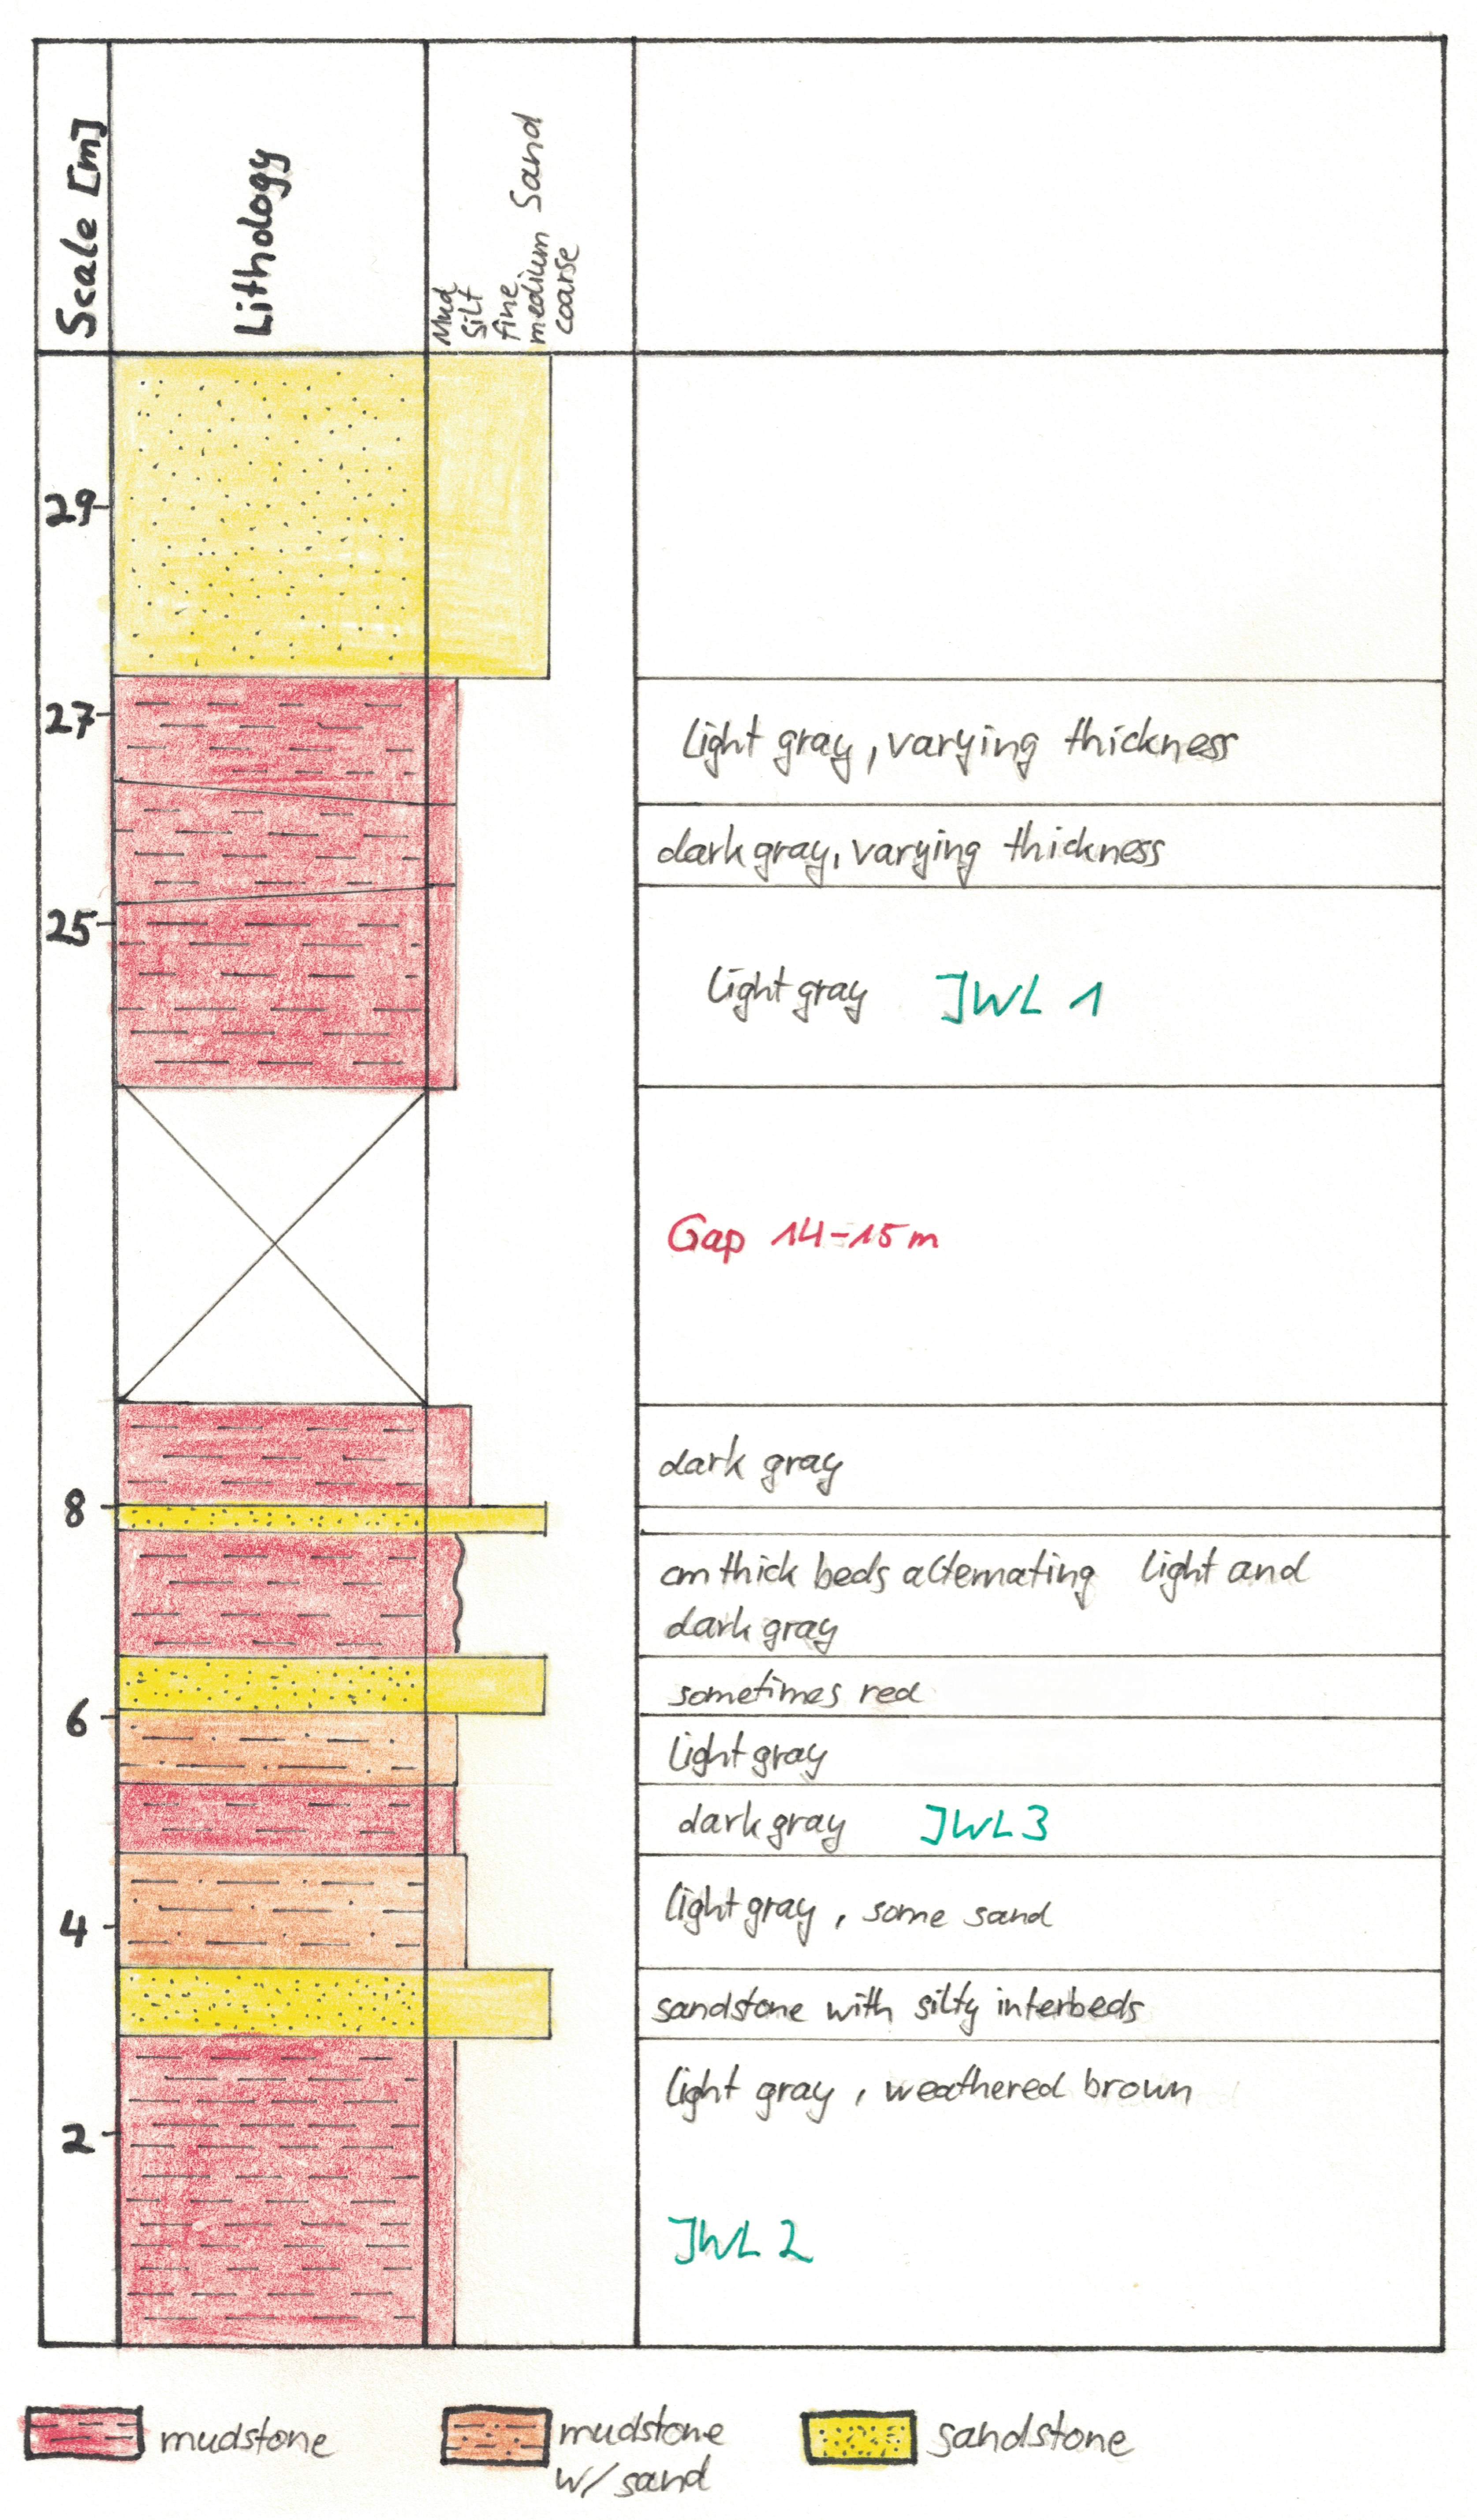
\includegraphics[width=0.5\textwidth]{img/L1_log.jpg}
    \caption{Stratigraphic log of the outcrop where samples JWL 1, 2 and 3 were taken. The outcrop
    is interrupted by an overgrown gap.}
    \label{fig:log_L1}
\end{figure}

% \begin{figure}
%     \centering
%     \fbox{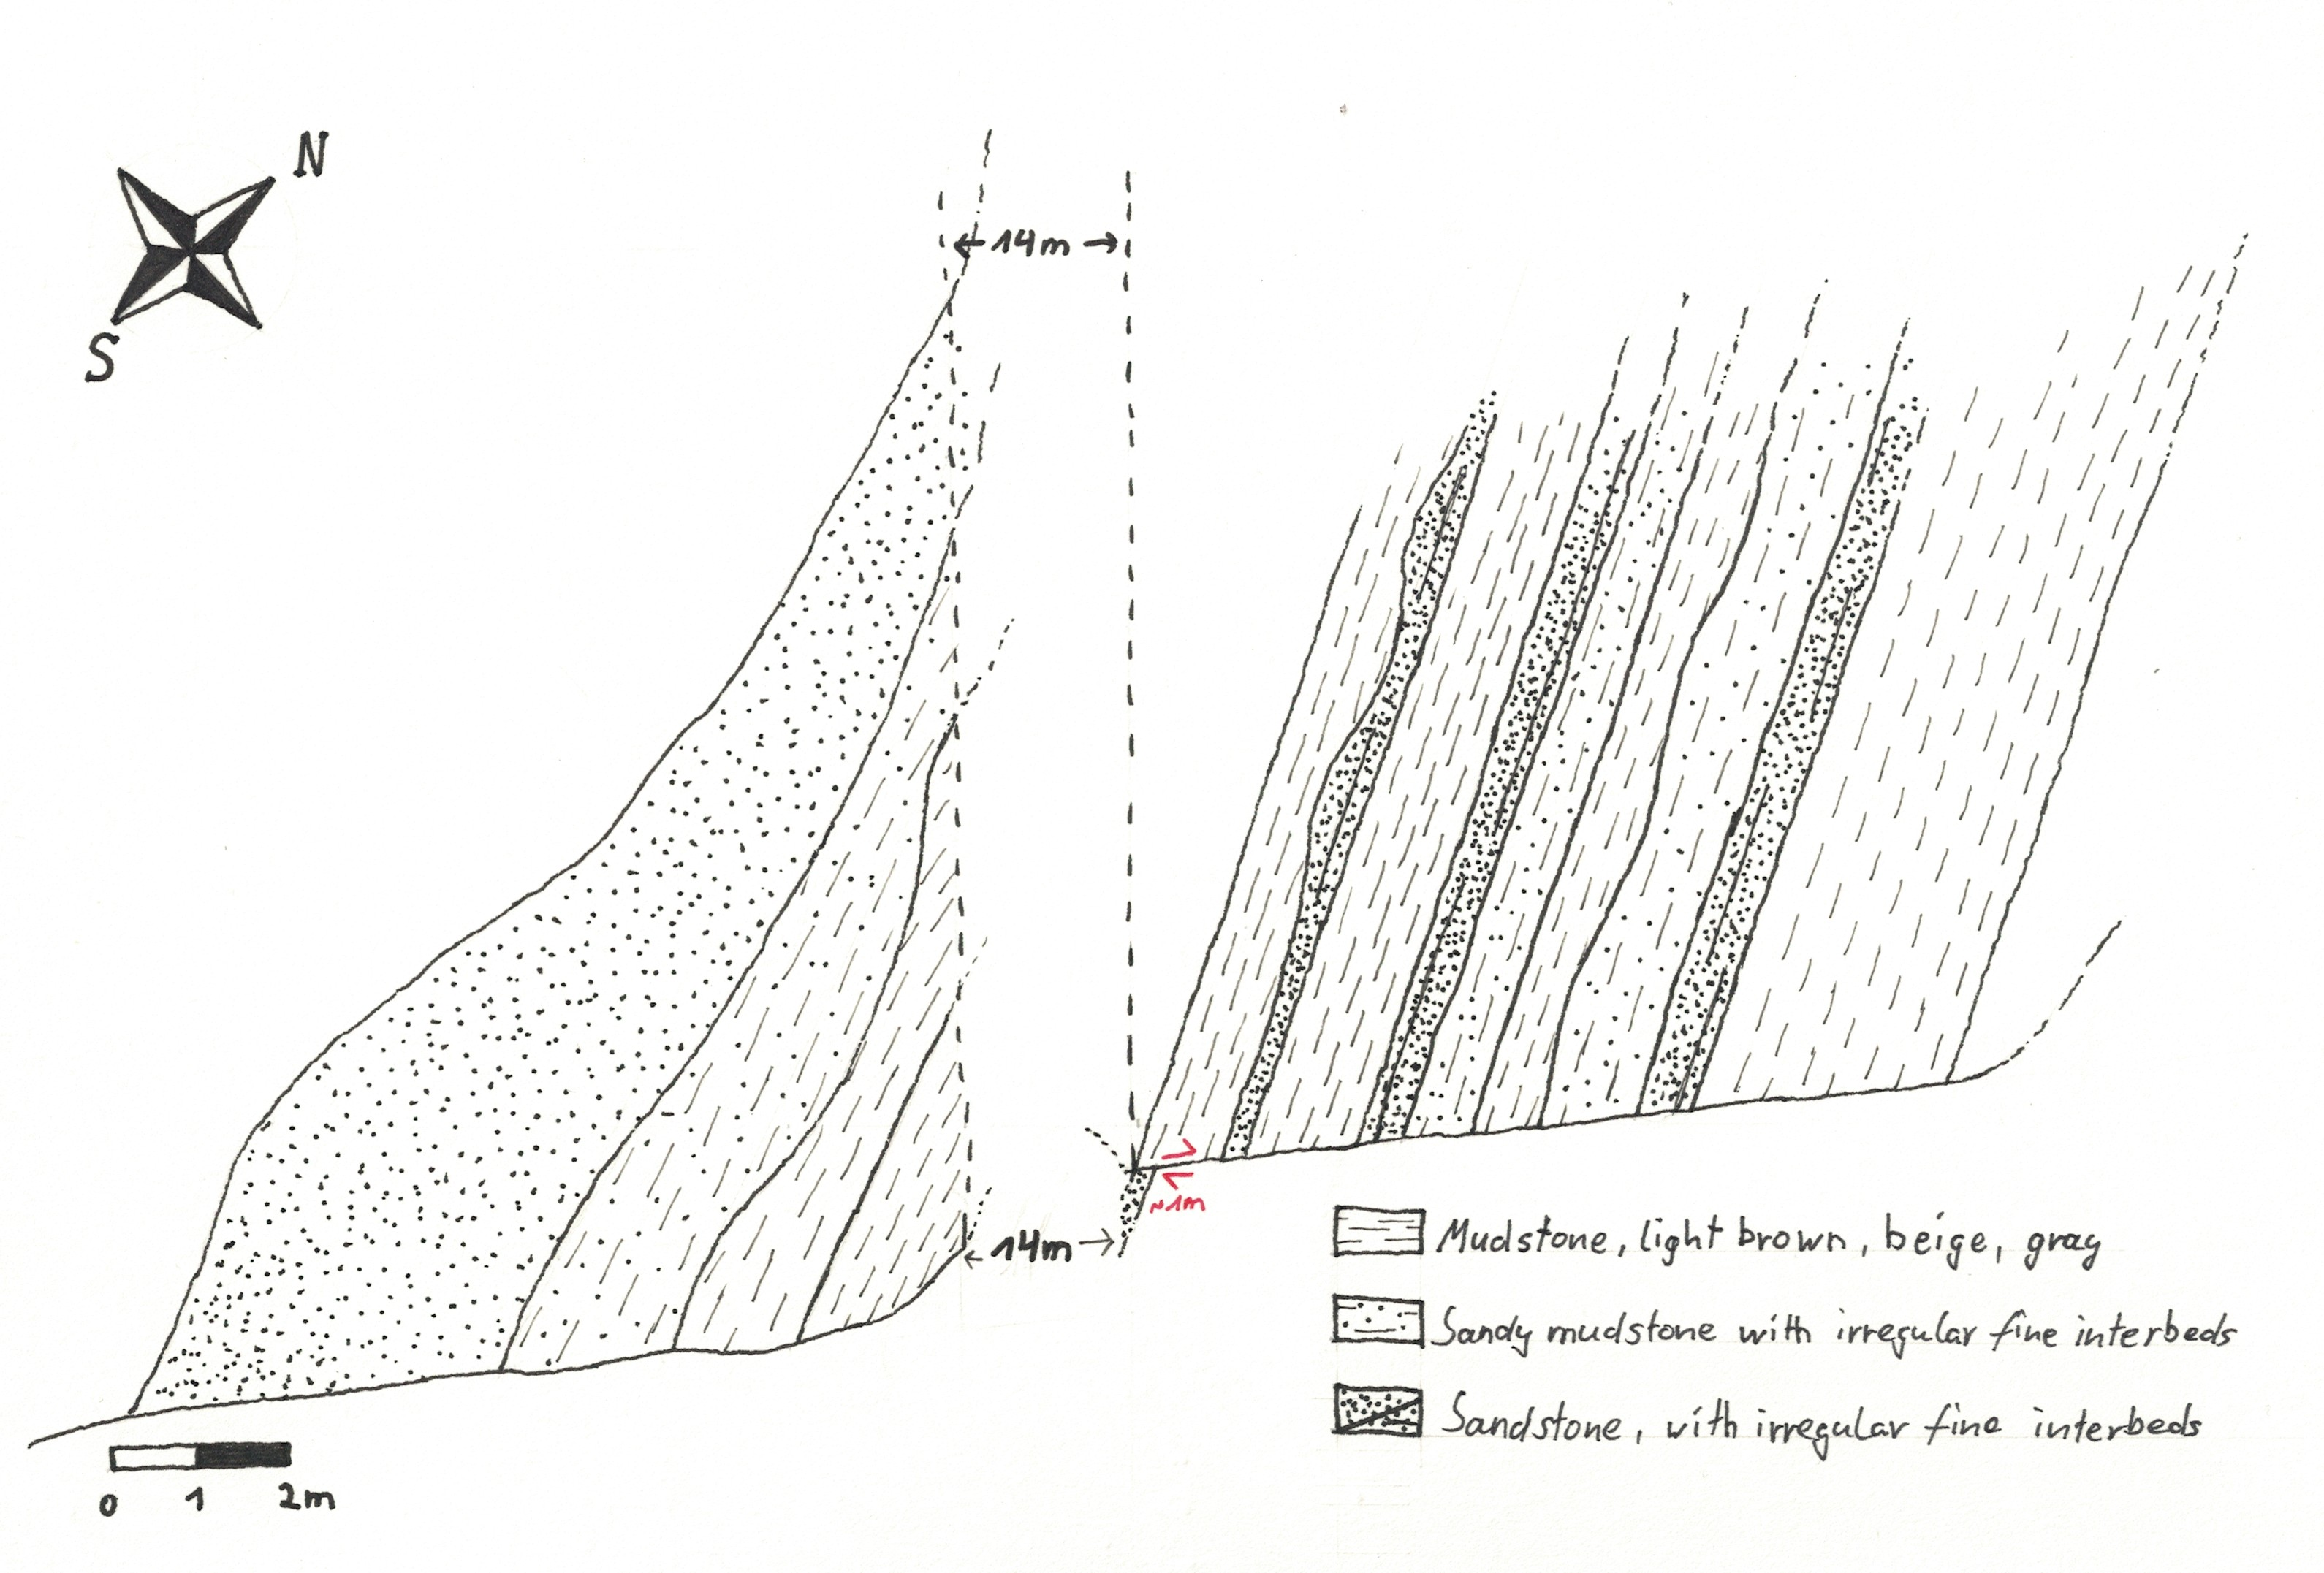
\includegraphics[width=0.95\textwidth]{img/loc_1_sketch.jpg}}
%     \caption{Sketch of the outcrop logged in \protect\cref{fig:log_L1}.
%     Bedding dips 200/65 in the right section. Dip is less clear in the more deformed left section.
%     Younging from right to left.}
%     \label{fig:loc_1_sketch}
% \end{figure}
